\begin{figure} [htbp]
  \begin{subfigure}[b]{.49\textwidth}
   \centering
   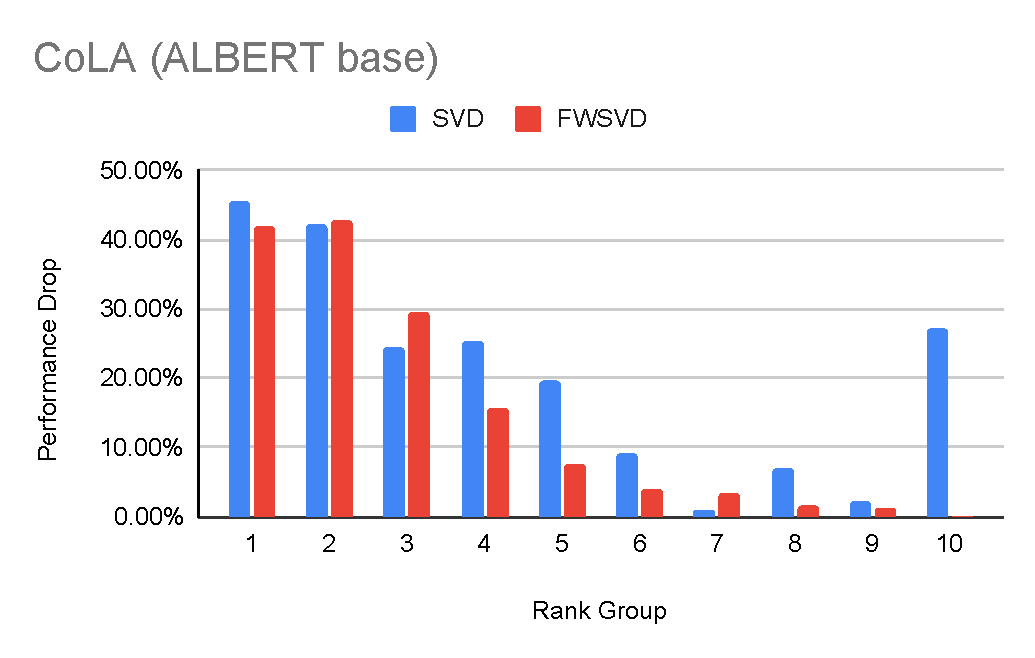
\includegraphics[width=\textwidth]{figures/group_truncation/CoLA_ALBERT_base.pdf}
       \caption{}
       \label{fig:rank_group_cola_albert}
       \end{subfigure}
\begin{subfigure}[b]{.49\textwidth}
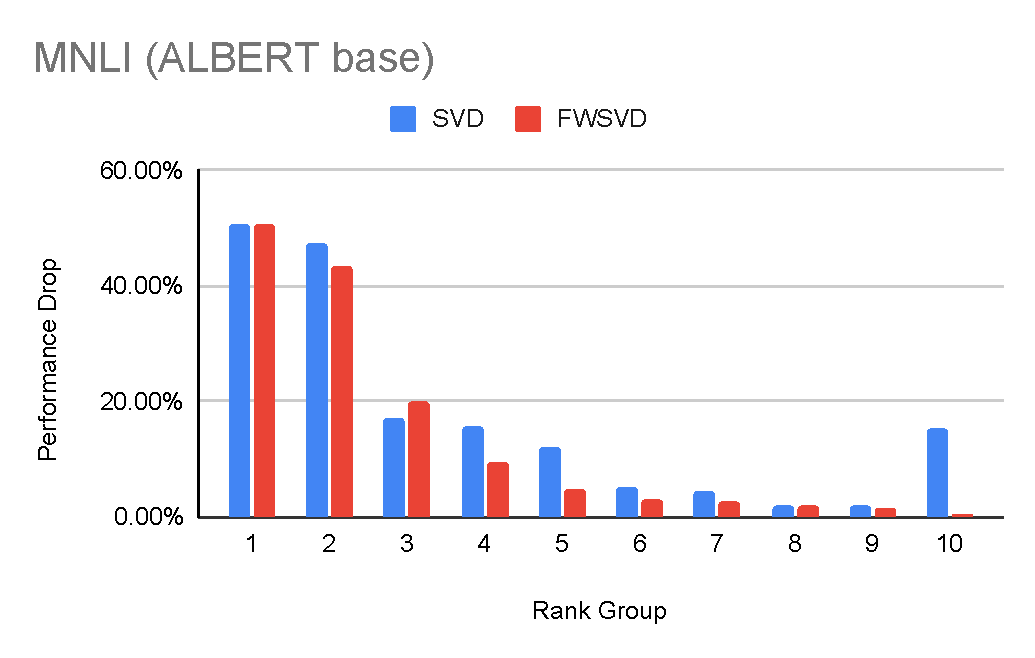
\includegraphics[width=\textwidth]{figures/group_truncation/MNLI_ALBERT_base.pdf}
\centering
  \caption{}
   \label{fig:rank_group_mnli_albert}
\end{subfigure}
\begin{subfigure}[b]{.49\textwidth}
   \centering
   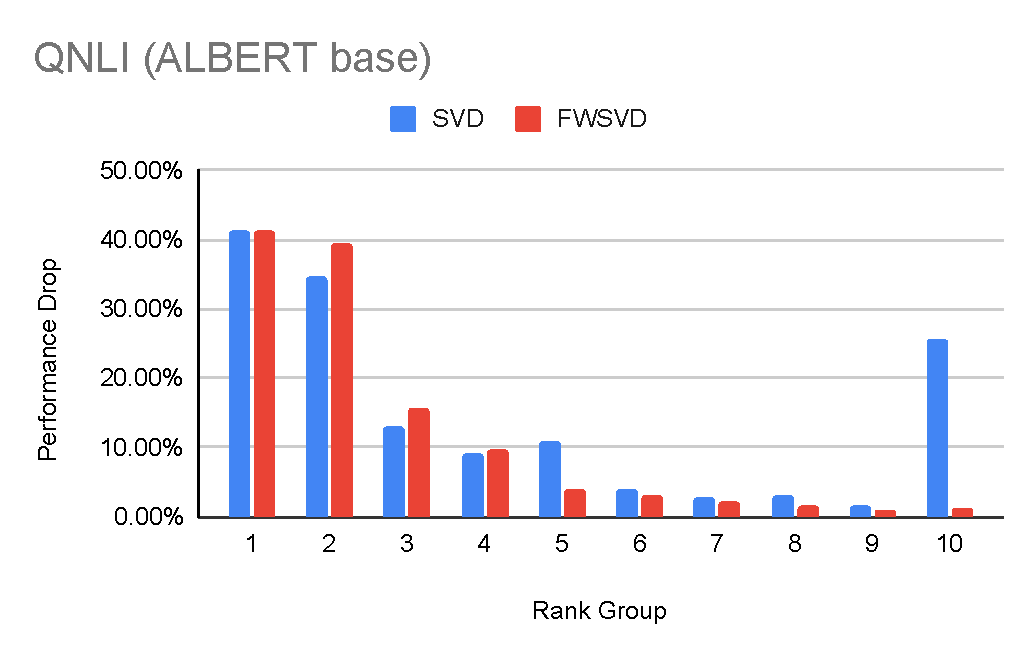
\includegraphics[width=\textwidth]{figures/group_truncation/QNLI_ALBERT_base.pdf}
       \caption{}
       \label{fig:rank_group_qnli_albert}
\end{subfigure}
\begin{subfigure}[b]{.49\textwidth}
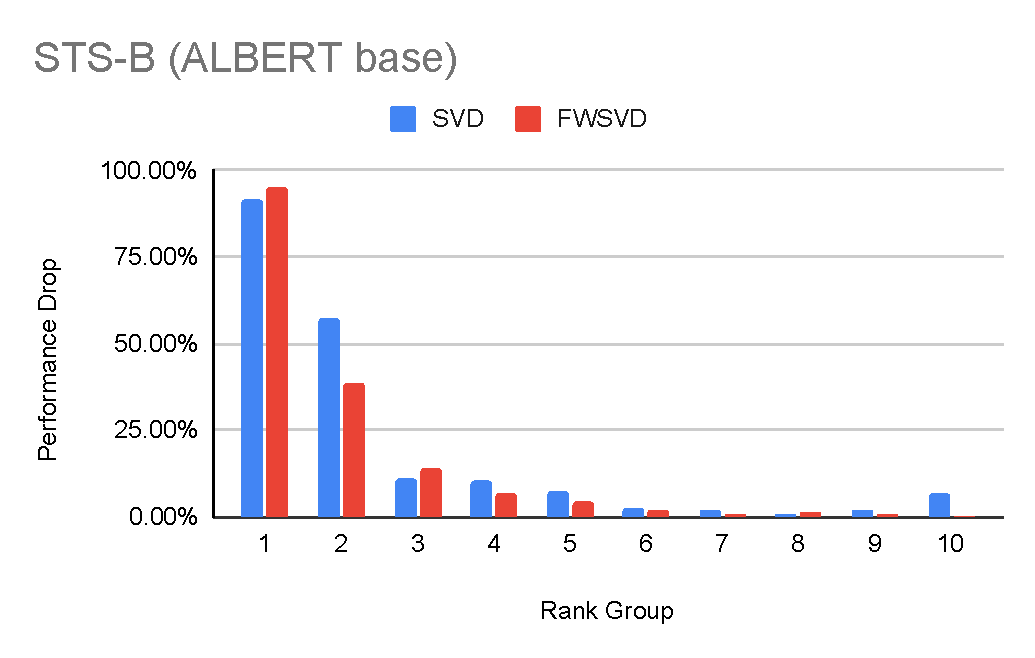
\includegraphics[width=\textwidth]{figures/group_truncation/STS-B_ALBERT_base.pdf}
\centering
  \caption{}
   \label{fig:rank_group_stsb_albert}
\end{subfigure}
\begin{subfigure}[b]{.49\textwidth}
   \centering
   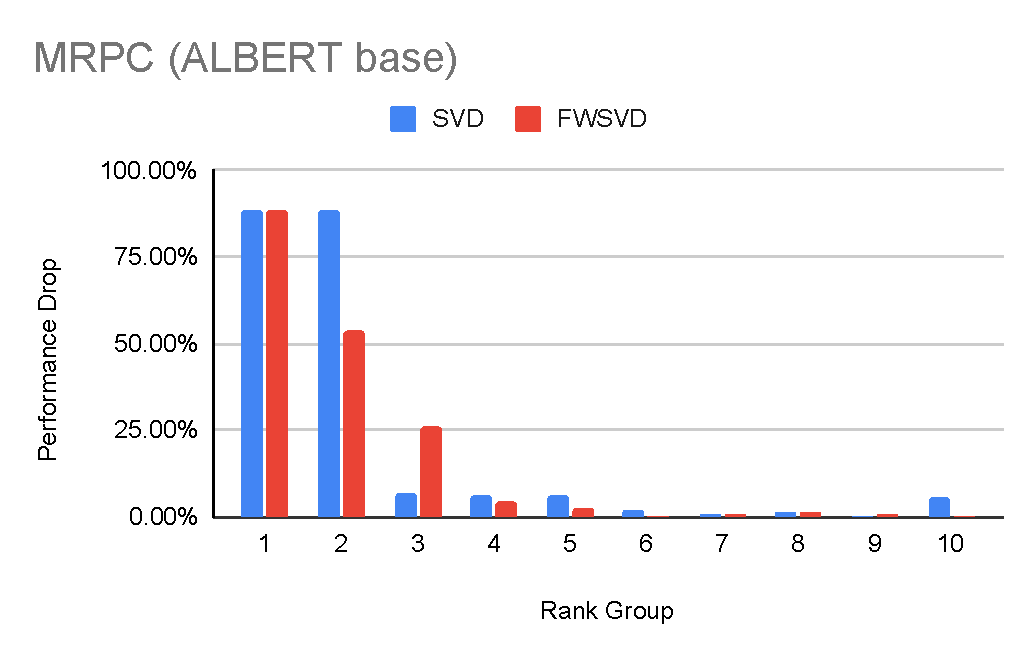
\includegraphics[width=\textwidth]{figures/group_truncation/MRPC_ALBERT_base.pdf}
       \caption{}
       \label{fig:rank_group_mrpc_albert}
       \end{subfigure}
\begin{subfigure}[b]{.49\textwidth}
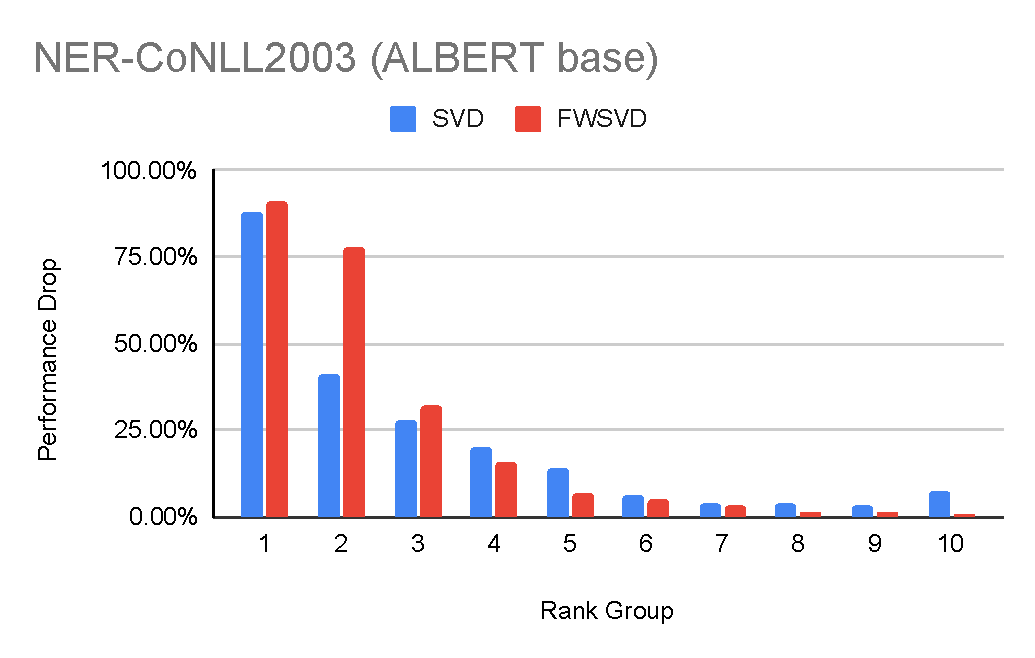
\includegraphics[width=\textwidth]{figures/group_truncation/NER-CoNLL2003_ALBERT_base.pdf}
\centering
  \caption{}
   \label{fig:rank_group_ner_albert}
\end{subfigure}
\begin{subfigure}[b]{.49\textwidth}
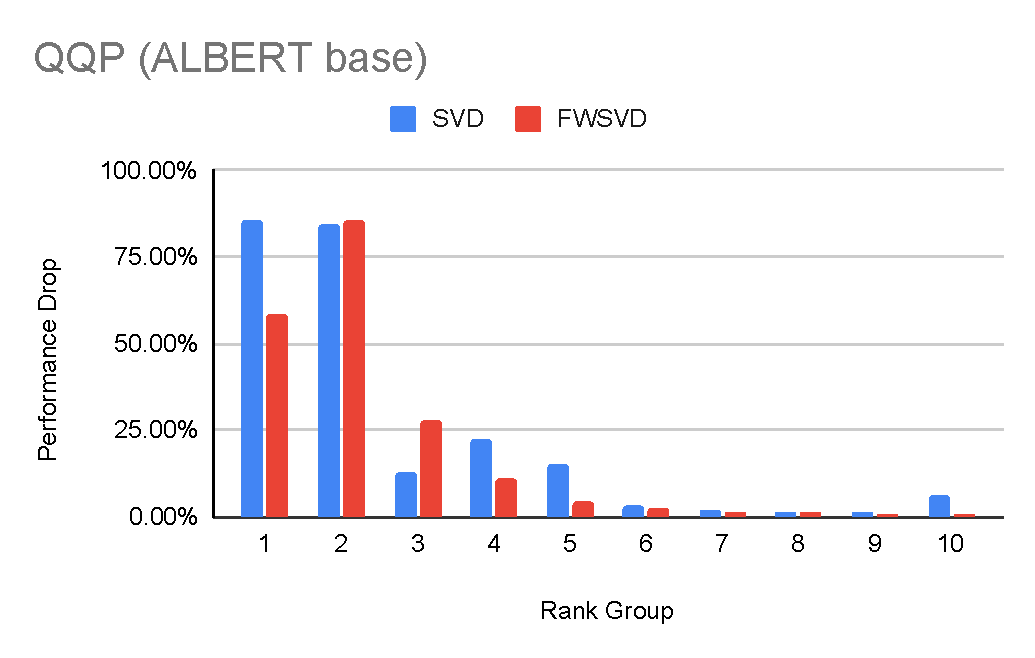
\includegraphics[width=\textwidth]{figures/group_truncation/QQP_ALBERT_base.pdf}
\centering
  \caption{}
   \label{fig:rank_group_qqp_albert}
\end{subfigure}
\begin{subfigure}[b]{.49\textwidth}
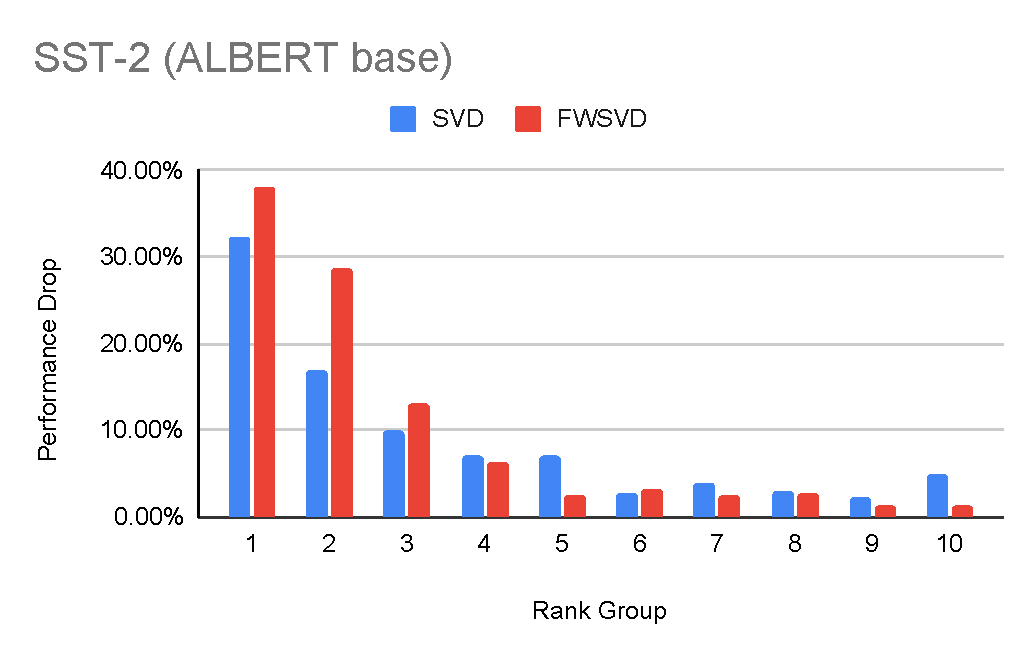
\includegraphics[width=\textwidth]{figures/group_truncation/SST-2_ALBERT_base.pdf}
\centering
  \caption{}
   \label{fig:rank_group_sst2_albert}
\end{subfigure}
\caption{The grouped rank truncation experiment. The experiments are the same with Figure \ref{fig:remove_group:drop}, but we use ALBERT$_{base}$ (11.7M parameters) model for this figure.
}
\label{fig:truncation_albert}
\end{figure}